%%%%%%%%%%%%%%%%%%%%%%%%%%%%%%%%%%%%%%%%%
% Software engineering project report
%%%%%%%%%%%%%%%%%%%%%%%%%%%%%%%%%%%%%%%%%


\documentclass{article}
\usepackage{fancyhdr} % Required for custom headers
\usepackage{lastpage} % Required to determine the last page for the footer
\usepackage{extramarks} % Required for headers and footers
\usepackage[usenames,dvipsnames]{color} % Required for custom colors
\usepackage{graphicx} % Required to insert images
\usepackage{listings} % Required for insertion of code
\usepackage{courier} % Required for the courier font
\usepackage{hyperref}
\usepackage{graphicx}
\usepackage[english]{babel}
\usepackage{amsmath,mathtools}
\usepackage[nottoc]{tocbibind}

% Margins
\topmargin=-0.45in
\evensidemargin=0in
\oddsidemargin=0in
\textwidth=6.5in
\textheight=9.0in
\headsep=0.25in
\linespread{1.1} % Line spacing

\hypersetup{
  pdftitle={\@hmwkTitle}, 
  pdfauthor={\@hmwkAuthorName},
  pdfsubject={\@hmwkClass}
}

% Set up the header and footer
\pagestyle{fancy}
\lhead{\hmwkAuthorName} % Top left header
\chead{\hmwkClass: \hmwkTitle} % Top center head
\rhead{\hmwkAuthorName} % Top right header
\lfoot{\lastxmark} % Bottom left footer
\cfoot{} % Bottom center footer
\rfoot{Page\ \thepage\ of\ \protect\pageref{LastPage}} % Bottom right footer
\renewcommand\headrulewidth{0.4pt} % Size of the header rule
\renewcommand\footrulewidth{0.4pt} % Size of the footer rule

\setlength\parindent{0pt} % Removes all indentation from paragraphs

 
%----------------------------------------------------------------------------------------
%	CODE INCLUSION CONFIGURATION
%----------------------------------------------------------------------------------------

\definecolor{MyDarkGreen}{rgb}{0.0,0.4,0.0} % This is the color used for comments
\lstloadlanguages{C++} % Load C++ syntax for listings, for a list of other languages supported see: ftp://ftp.tex.ac.uk/tex-archive/macros/latex/contrib/listings/listings.pdf
\lstset{language = C++, % C++ code Dos
        frame=single, % Single frame around code
        basicstyle=\small\ttfamily, % Use small true type font
        keywordstyle=[1]\color{Blue}\bf, % C++ functions bold and blue
        keywordstyle=[2]\color{Purple}, % C++ function arguments purple
        keywordstyle=[3]\color{Blue}\underbar, % Custom functions underlined and blue
        identifierstyle=, % Nothing special about identifiers                                         
        commentstyle=\usefont{T1}{pcr}{m}{sl}\color{MyDarkGreen}\small, % Comments small dark green courier font
        stringstyle=\color{Purple}, % Strings are purple
        showstringspaces=false, % Don't put marks in string spaces
        tabsize=5, % 5 spaces per tab
        %
        % Put standard C++ functions not included in the default language here
        morekeywords={rand},
        %
        % Put C++ function parameters here
        morekeywords=[2]{on, off, interp},
        %
        % Put user defined functions here
        morekeywords=[3]{test},
       	%
        morecomment=[l][\color{Blue}]{...}, % Line continuation (...) like blue comment
        numbers=left, % Line numbers on left
        firstnumber=1, % Line numbers start with line 1
        numberstyle=\tiny\color{Blue}, % Line numbers are blue and small
        stepnumber=5 % Line numbers go in steps of 5
}

% Creates a new command to include a c++ script, the first parameter is the filename of the script (without .cpp), the second parameter is the caption
\newcommand{\codescript}[2]{
\begin{itemize}
\item[]\lstinputlisting[caption=#2,label=#1]{#1.cpp}
\end{itemize}
}
%create template for command prompt
\lstdefinestyle{DOS}
{
    backgroundcolor=\color{black},
    basicstyle=\scriptsize\color{white}\ttfamily
}
%----------------------------------------------------------------------------------------
%	DOCUMENT STRUCTURE 
%----------------------------------------------------------------------------------------

% Header and footer for when a page split occurs within a problem environment
\newcommand{\enterProblemHeader}[1]{
\nobreak\extramarks{#1}{#1 continued on next page\ldots}\nobreak
\nobreak\extramarks{#1 (continued)}{#1 continued on next page\ldots}\nobreak
}

% Header and footer for when a page split occurs between problem environments
\newcommand{\exitProblemHeader}[1]{
\nobreak\extramarks{#1 (continued)}{#1 continued on next page\ldots}\nobreak
\nobreak\extramarks{#1}{}\nobreak
}

\setcounter{secnumdepth}{0} % Removes default section numbers
\newcounter{homeworkProblemCounter} % Creates a counter to keep track of the number of problems

\newcommand{\homeworkProblemName}{}
\newenvironment{homeworkProblem}[1][Part \arabic{homeworkProblemCounter}]{ % Makes a new environment called homeworkProblem which takes 1 argument 
\stepcounter{homeworkProblemCounter} % Increase counter for number of problems
\renewcommand{\homeworkProblemName}{#1} % Assign \homeworkProblemName the name of the problem
\section{\homeworkProblemName} % Make a section in the document with the custom problem count
\enterProblemHeader{\homeworkProblemName} % Header and footer within the environment
}{
\exitProblemHeader{\homeworkProblemName} % Header and footer after the environment
}

\newcommand{\problemAnswer}[1]{ % Defines the problem answer command with the content as the only argument
\noindent\framebox[\columnwidth][c]{\begin{minipage}{0.98\columnwidth}#1\end{minipage}} % Makes the box around the problem answer and puts the content inside
}


\newcommand{\homeworkSectionName}{}
\newenvironment{homeworkSection}[1]{ % New environment for sections within homework problems, takes 1 argument - the name of the section
\renewcommand{\homeworkSectionName}{#1} % Assign \homeworkSectionName to the name of the section from the environment argument

\subsection{\homeworkSectionName} % Make a subsection with the custom name of the subsection
\enterProblemHeader{\homeworkProblemName\ [\homeworkSectionName]} % Header and footer within the environment
}{
\enterProblemHeader{\homeworkProblemName} % Header and footer after the environment
}

%----------------------------------------------------------------------------------------
%	NAME AND CLASS SECTION
%----------------------------------------------------------------------------------------

\newcommand{\hmwkTitle}{Laplace Spectral Representation} % Assignment title
\newcommand{\hmwkDueDate}{,\ January\ 14,\ 2015} % Due date
\newcommand{\hmwkClass}{Software Engineering  } % Course/class
\newcommand{\hmwkClassTime}{} % Class/lecture time
\newcommand{\hmwkClassInstructor}{ Yohan Fougerolle } % Teacher/lecturer
\newcommand{\hmwkAuthorName}{Pramita Winata } % Your name

%----------------------------------------------------------------------------------------
%	TITLE PAGE
%----------------------------------------------------------------------------------------

\title{
\vspace{2in}
\textmd{\textbf{\hmwkClass:\ \hmwkTitle}}\\
\normalsize\vspace{0.1in}\small{Due\ on\ \hmwkDueDate}\\
\vspace{0.1in}\large{\textit{\hmwkClassInstructor\ \hmwkClassTime}}
\vspace{3in}
}

\author{\textbf{\hmwkAuthorName} \\ Dragutin}
%\date{Sunday,\ December\ 21,\ 2014}

%----------------------------------------------------------------------------------------

\begin{document}

\maketitle
%----------------------------------------------------------------------------------------
%	TABLE OF CONTENTS
%----------------------------------------------------------------------------------------

%\setcounter{tocdepth}{1} % Uncomment this line if you don't want subsections listed in the ToC

\newpage
\tableofcontents
\clearpage

\newpage
\section{Introduction}
  This application is done as part of Software Engineering course project.  The aim of this project is to show basic Laplace spectral representation and to implement C++ programming skill.
 It is developed under Qt IDE 5.3.0 using OpenGL and Eigen library. I will discuss the project implementation in two main sections; basic laplace representation and application development. Paper \cite{laplacemesh} is mainly used in the Laplace implementation. The development of the application is the extension of the existing project where improvement in the Graphical User Interface (GUI) is done and Laplacian representation is cooperated. 
 
 
\begin{homeworkProblem}[Section \arabic{homeworkProblemCounter} - Basic Laplace representation]
This part of the implementation is to satisfied the second and third objectives of the project where we need to implement section 2.1 of paper \cite{latexcompanion} by using the $Neighbourmesh$ class given in $Meshloader.pro$. Inside $Meshloader.pro$, I can already find many extremely useful function that can be used to implement \cite{latexcompanion}, especially functions in $Neighbourmesh.cpp$. Eigen library \cite{eigenlib} also very useful on implementing this project, especially $SparseMatrix$ class that I use to store the cotangent weight and the Laplace matrix. 

\begin{figure}[h!]
  \centering
  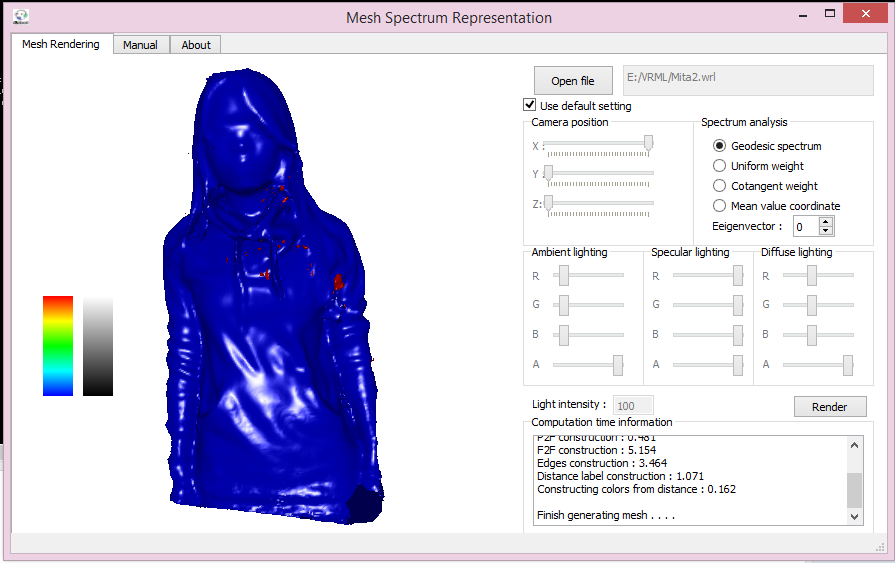
\includegraphics[scale=0.3]{3DRepresentation.png}
  \caption{3D Representation}
  \label{fig:mita}
\end{figure}
The Figure\ref{fig:mita}  below is a 3D representation of me. The $wrl$ file is generated with kinect in 3D lab in IUT.
\\ 

To start the implementation, I need to understand what is mesh representation. Mesh representation in 3D is a way to represent 3D objects in a computer. Construction of a data structure that can be recognize by a computer for it to manipulate, analyze 3d objects. There are many 3D representation has been developed until now, such as boundary representations, solid representations, image-based representation, and etc. Each of the representation has also subsections of representing 3D objects. For this project, we will deal with 3D boundary triangle mesh representation. \\ 

\begin{figure}[h!]
  \centering
  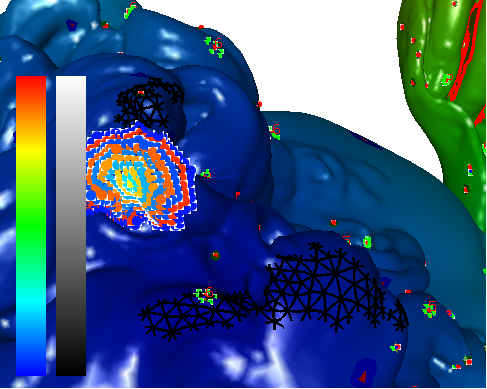
\includegraphics[scale=0.5]{TriangularMesh.png}
  \caption{Triangular mesh Representation}
  \label{fig:triangularmesh}
\end{figure}

\codescript{DrawTriangularMesh}{ DrawTriangularMesh function in $LaplacianMesh.cpp$}
In this function, Glut function from OpenCV is used and also notice that I only iterates 100 times since the purpose is just to illustrate triangular mesh . 
\\
Triangular meshes representation of a 3D point consists of a set of triangles built from the given point and its neighbor. We will have an 'umbrella' like shape for each of the 3D points. In the $Meshloader.pro$, data structure to read $wrl$ file has already being built. The necessary and useful calculation such as getting the neighborhood vertices's and faces' has already being computed and nicely set. \\

The next step is to understand basic Laplace mesh representation. In Laplacian framework, each vertex is represented with consideration to its neighbors unlike Cartesian coordinates that only represent the spatial location. Laplacian meshes store the location of a vertex relative to its neighboring vertices. This is useful when the information of object's shape are important for example when deforming the object itself. With Laplacian mesh representation, we can use manipulate one vertex, as known as 'anchor' based on \cite{latexcompanion},  to have the overall objects deformed in a correct way. In regular meshes, for example, we need to manipulate many vertices to get this done.  \\

In Laplacian framework, we need to obtain a variable for each vertex that represent its location based on its immediate neighbours' vertices. This variable is called $differential$ or $\delta-coordinates$ of each vertex. In paper \cite{laplacemesh} the $differential$ or $\delta-coordinates$ of $v_i$ is the difference between the absolute coordinates of $v_i$ and the center of mass of its immediate neighbors in the mesh. 
    $$
    \delta_i = (\delta_i^{(x)} , \delta_i^{(y)}, \delta_i^{(z)} ) = v_i - \frac{1}{d-i} \sum_{j\in N(i)} v_j ,
    $$
    where $N(i) = {j |(i,j) \in E}$ and $d_i = |N(i)|$ is the number of immediate neighbors of $i$ ( the degree or valence of $i$).

It is important to understand that each vertex will have weight correspond to each of its neighbor. In this project, I will implement three method to get the weight of the vertex. These method are uniform weight, cotangent weight, and mean-value-coordinate.


\subsection{Uniform weight}
In uniform weight method, the weight of each vertex depends on the size of its immediate neighbor. According to \cite{laplacemesh}, the symmetric Laplace Matrix can be denoted by: \\
\[
L_{s_{ij}} =
  \begin{cases}
     d_i & \text{if }i=j \\
     -1  & \text{if } (i,j)\in\varepsilon \\
     0   & otherwise
  \end{cases}
\]


In implementing this, I created new class $LaplaceMesh.cpp$, this class contains the calculation for this. Below are the header file of $LaplaceMesh.cpp$.

\codescript{laplacianMeshHeader}{Header file for $LaplaceMesh$ class}

\codescript{GetLaplacianUniformWeight}{ Function to calculate Laplacian Matrix with uniform weight}  

From here, I can construct the Laplace matrix from the Laplace definition above. The differential coordinates for each of vertex can be obtained by multiplying the Laplacian by the original coordinates. It represents the difference between the average position of its neighbors and the vertex's actual position, which corresponds to local detail. 
\\

In order to check whether the matrix and vector generated are fine, I created two function $SaveMatrix$ and $SaveVector$ in $Useful$ class. These function will store the corresponding matrix or vector to a text file in a given path. 
\codescript{SaveMatrixVector}{ Function to save matrix and vector to a text file }  

I tested the the function with $Icosaedron.wrl$ file. The matrix generation takes 2.452 seconds. The snipplet of Laplace matrix generated is shown in Figure \ref{fig:laplacematrix}.
 
\begin{figure}[h!]
   \centering
   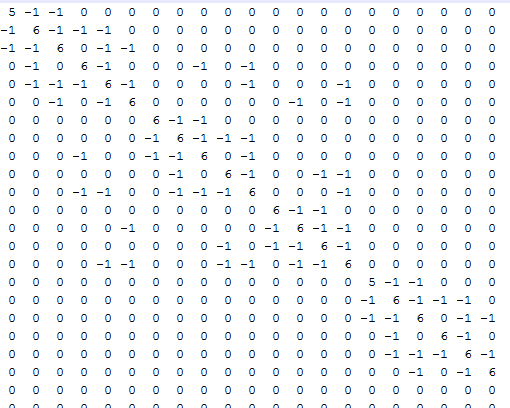
\includegraphics[scale=1]{LaplaceMatrix.png}
   \caption{Laplace matrix for $Icosaedron.wrl$ }
   \label{fig:laplacematrix}
\end{figure}
It is realized that 
$$
  L_s * vertex_{i} = D \delta_i
$$
where $D$ is diagonal matrix with $D_ii = d_i$. Eigen decomposition then done in Laplace matrix. When eigen decomposition is done on the Laplace matrix, one eigenvector can be chosen to be our new set of weighted-vertices.

\codescript{CalculateEigenDecomposition}{ Function to calculate eigen decomposition of Laplacian Matrix} 

\begin{figure}[h!]
   \centering
   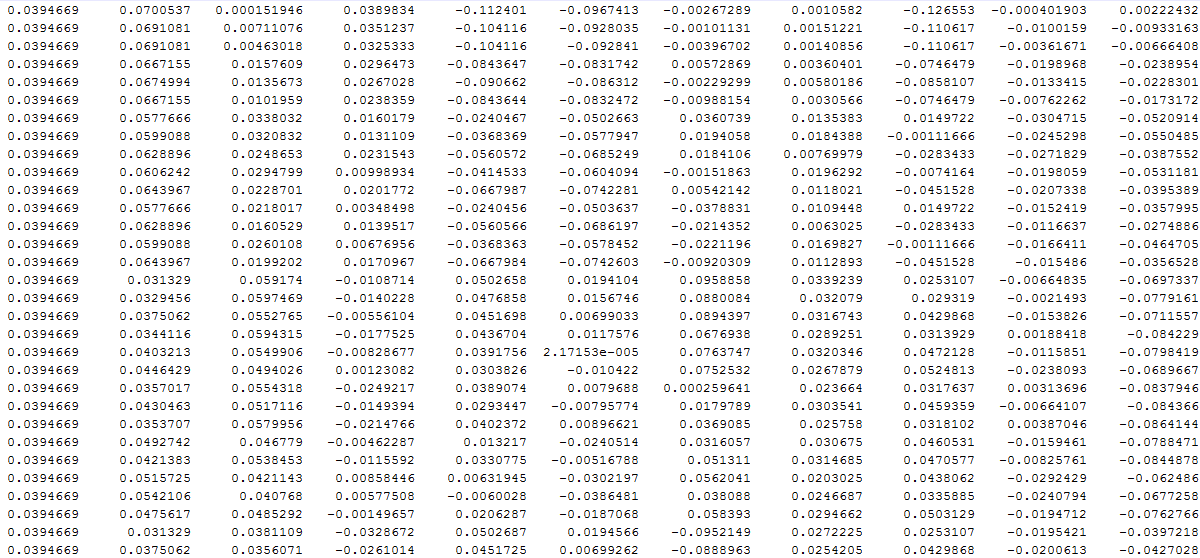
\includegraphics[scale=0.5]{EigenVectors.png}
   \caption{ Computed eigenvectors }
   \label{fig:eigenvetorsmatrix}
 \end{figure}

I utilize the $EigenSolver$ class from Eigen library in C++. The implementation is very straightforward. I can just instantiate the solver with specifying the datatype of Matrix to be solved, in this case $MatrixXd$, and call the $compute$ function. Eigenvectors and eigenvalues of the matrix will be stored in a $MatrixXd$. Figure \ref{fig:eigenvetorsmatrix} shows the snipplet of the eigenvectors' matrix. This is stored in text file for later references.

 From here, I get one real eigenvector. This eigenvector will represent new weighted value of the vertices. Figure \ref{fig:eigenvectorchosen} shows the snipplet of the eigenvectors' matrix. This is stored in text file for later references. \\ 
 
\begin{figure}[h!]
   \centering
   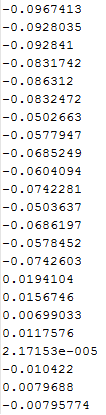
\includegraphics[scale=0.5]{EigenVectorChosen.png}
   \caption{Sniplet of eigen vector chosen }
   \label{fig:eigenvectorchosen}
 \end{figure}
 

 
 
After obtaining this new set of values, I build a colormap to illustrate the eigen decomposition of the mesh.  
\\
\codescript{BuildColorMap}{ Function to get the new colormap based on the eigen vector of Laplace matrix }
Generating the color map takes s
\begin{figure}[h!]
   \centering
   \label{fig:eigendecomposedos}
   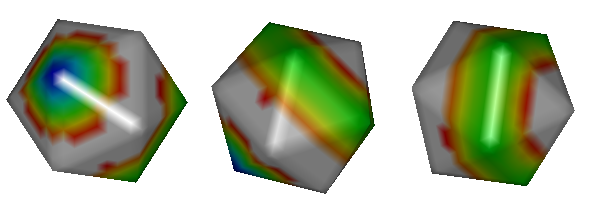
\includegraphics[scale=1]{EigenvectorMeshCol4.png}
   \caption{ New mesh colormap based on the chosen $4_th$ column eigenvector }	
 \end{figure}

Total time to finish the whole process is shown in Figure \ref{fig:computationtimeuniform}.
\begin{figure}[h!]
   \centering
   \label{fig:computationtimeuniform}
	\begin{lstlisting}[style=DOS]
	READ FILE
	Extension=WRL
	Reading IV/VRML
	Loading time :0.033 s
	P2P construction :0.007 s
	P2F construction :0.004 s
	F2F construction :0.042 s
	Egdes construction :0.023 s
	Laplacian matrix can be found in C:/Users/User/Documents/Master_VIBOT/Semester1/laplacian.txt
	Calculating laplacian matrix: 2.498 s
	Computing Eigen decomposition
	Calculating eigen decomposition: 165.906 s
	Building eigen color map: 0.011 s
	\end{lstlisting}
	\caption{Computation time}	
 \end{figure}

It is also worth notes that the size of the $.wrl$ file used is playing a huge role in this implementation, especially the size of the vertices inside it. I have encountered many problem in regards of this. First, the problem when instantiating the Laplace matrix using $MatrixXd$. Laplace matrix needs to be instantiated as $n x n$ matrix, with $n$ is the number of vertices in the mesh. If this variable gets too big, Qt will not be able to handle it. I am running the Qt with MinGW 32 bit, the maximum memory size can be allocated is 4 GB. Mesh with total vertices 100.000, will need to instantiate  100.000 x 100.000 size of Matrix, which is far greater than the limit of the application. \\
There are three solution for this : 
\begin{enumerate}
\item Memory increment \\
Increasing the memory by change the Qt compiler to get be work on MinGw 64 bit. These will also require changing the Qt Desktop application to be 64 bit version and setting everything up again. 
\item Code modification \\
Changing the way Laplace matrix instantiated could be a solution. In Eigen library, $SparseMatrix$ class can be used to store Laplacian since Laplace matrix is extremely sparse ( most of the value is zero ). It can be instantiated with a huge number without taking much memory. However this solution has one big drawback, $Sparse$ matrix class in Eigen is not supported in $EigenSolver$. External library like ARPACK needs to be cooperated in Qt.
\item Data modification \\
The easiest and more practical solution is to change the data having a reasonable amount of vertices. This what I have chosen to be the solution for this project. Meshes like dolphin, Icoheadral, or mannequin can be computed in 32 bit compiler. This is not the best solution but it is an acceptable solution in my opinion.
\end{enumerate}

\subsection{Cotangent weight}
The weight use previously, is improved by \cite{cotangentweight}
We can also generate the Laplacian matrix by using the cotangent weight instead of its uniform weight . 
$$
    \delta_i^c = \frac{1}{|\Omega_i|} \sum_{j\in} {\frac{1}{2} ( cot \alpha_{ij} +  cot \beta_ij)  (v_i - v_j) },
$$
where $|\Omega_i|$ is the size of the Voronoi cell of $i$ and $\alpha_{ij}$, $\beta_{ij}$ denote
the two angles opposite of edge $(i, j)$ 
 \begin{figure}[h!]
   \centering
   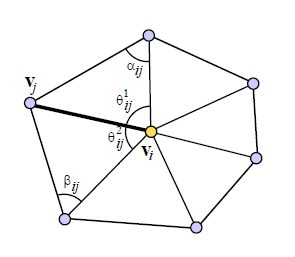
\includegraphics[scale=0.5]{CotangentWeight.png}
   \caption{Cotangent weight }
   \label{fig:cotangentweightill}
 \end{figure}

Thus I get, the cotangent weight: \\
$$
 \omega_ij = \frac{1}{2} ( cot \alpha_{ij} +  cot \beta_ij)
$$
After computing$\omega_ij$, we can get the Laplacian matrix, $L$	,that comprises :
\begin{itemize}
\item $L_(ij) = \omega_ij$, if $i$ and $j$ are neighbors
\item $L_(ij) = 1$, if $i = j$ are neighbors
\item 0, everywhere else
\end{itemize}

\[
L_{s_{ij}} =
  \begin{cases}
     1 & \text{if }i=j \\
     \omega_ij  & \text{if } (i,j)\in\varepsilon \\
     0   & otherwise
  \end{cases}
\]


To compute the cotangent, I use the equation illustrated in \cite{cotangentweight}.

If we have a triangle with vertices $vi; vj ; vk$, the triangle area $A_{ijk}$ is defined by \cite{areatriangle}:
$$
A_{ijk} = \sqrt[2]{r(r-l_{ij})(r-l_{jk})(r-l_{ki})}
$$
where $r$ is the semiperimeter
$$
 r = \frac{1}{2}(l_{ij} + l_{jk} + l_{ki}).
$$
The law of cosines:
$$
 cos\alpha_{ij} = \frac{-l_{ij}^2 + l_{jk}^2 + l_{ki}^2}{2l_{jk}l_{ki}}.
$$
For sine:
$$
 sin \alpha_{ij} = \frac{2A_{ijk}}{l_{jk}l_{ki}}
$$
I can get the cotangent by:
$$
 cot \alpha_{ij} = = \frac{cos \alpha_{ij}}{in \alpha_{ij}}
$$
\codescript{CalculateCotangent}{ Function to calculate the cotangent of a triangle }

Before calculating the cotangent weight, I need to find the correct triangle to be passed in to $CalculateCotangent$, in another case find the other vertex that formed the face. I iterates the faces of the vertex, and find the faces that contains the edge we are having. Code below shows the function $CalculateCotangentWeight$ that compute this.

\codescript{CalculateCotangentWeight}{ Function to calculate the cotangent weight of the vertices }

After having the cotangent calculation, we can build the Laplace Matrix using the rule given previously. 

\codescript{GetLaplacianCotangentWeight}{ Function to construct Laplace matrix with cotangent weight }

Here is a sniplet of the Laplace matrix.
\begin{figure}[h!]
   \centering
   \label{fig:laplaceMatrixCotWeight}
   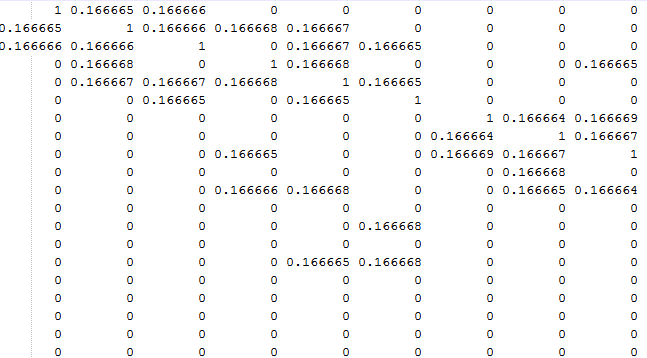
\includegraphics[scale=0.8]{LaplaceMatrixCotWeight.png}
   \caption{ Sniplet of Laplace matrix using Cotangent weight}	
 \end{figure}

The routine goes the same with previous method, we need to perform eigen decomposition and build the color map using the chosen eigenvector. I am using the same function built previously. The result of the color map is shown in Figure \ref{eigenmeshcotweight}
\begin{figure}[h!]
   \centering
   \label{fig:EigenVectorsCotangentWeight}
   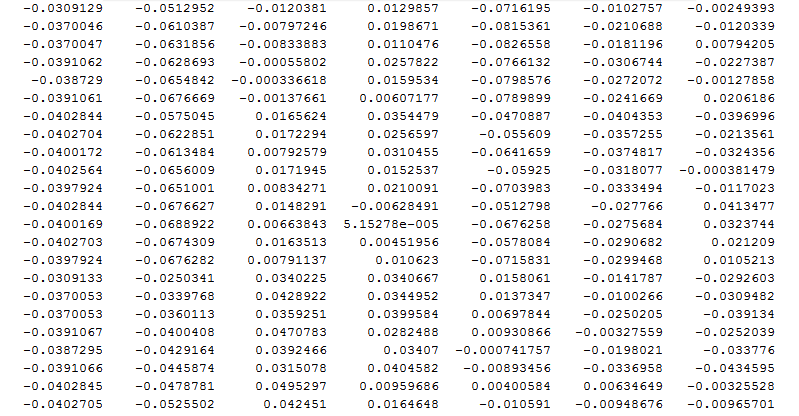
\includegraphics[scale=0.5]{EigenVectorsCotangentWeight.png}
   \caption{ Sniplet of eigenvectors matrix for the cotangent weight method}	
 \end{figure}
 \begin{figure}[h!]
    \centering
    \label{fig:EigenVectorChosenCotangentWeight}
    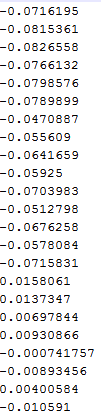
\includegraphics[scale=0.5]{EigenVectorChosenCotangentWeight.png}
    \caption{ Sniplet of the chosen eigenvector for the cotangent weight method}	
  \end{figure}

\begin{figure}[h!]
   \centering
   \label{fig:eigenmeshcotweight}
   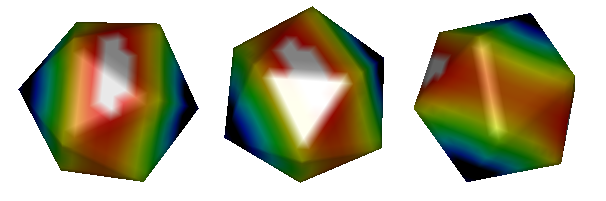
\includegraphics[scale=1]{EigenvectorMeshCotangentWeightCol4.png}
   \caption{ New mesh colormap based on the chosen $4_th$ column eigenvector for cotangent weight method }	
 \end{figure}

Total time to finish the whole process is shown in Figure \ref{fig:computationtimecotangent}.
\begin{figure}[h!]
   \centering
   \label{fig:computationtimecotangent}
	\begin{lstlisting}[style=DOS]
	READ FILE
	Extension=WRL
	Reading IV/VRML
	Loading time :0.019 s
	P2P construction :0.004 s
	P2F construction :0.002 s
	F2F construction :0.017 s
	Egdes construction :0.011 s
	Write Laplacian matrix to text file.
	Calculating laplacian matrix: 2.409 s
	Computing Eigen decomposition
	Calculating eigen decomposition: 167.785 s
	Building eigen color map: 0.014 s
	\end{lstlisting}
	\caption{Computation time}	
 \end{figure}

\subsection{Mean value coordinate}

Mean value coordinate is introduce by \cite{meanValue} to tackle the problem when the cotangent weights may be negative and in the case where the angle of the vertices is very big. \cite{meanValue} introduce this weight computation to solve this problem.
$$
    \delta_i^j = \frac{ \tan((\theta_{ij}^1)/2) + \tan((\theta_{ij}^2)/2)  ) }  {||v_i - v_j||},
$$
where $\theta$ is illustrated in Figure \ref{cotangentweightill}.

The Laplacian matrix, $L$, comprises:
\begin{itemize}
\item $L_(ij) = \omega_ij$, if $i$ and $j$ are neighbors
\item $L_(ij) = 1$, if $i = j$ are neighbors
\item 0, everywhere else
\end{itemize}

$$
 L_{s_{ij}} =\left\{\begin{matrix}
 1      ,  i=j\\  
 w_{ij} , (i,j)\in\varepsilon \\
 0      , otherwise) 
\end{matrix}\right.
$$

To compute the cotangent, I use the same method as in calculation cotangent computation illustrated in \cite{cotangentweight}.

\codescript{CalculateTangent}{ Function to calculate the tangent for mean value coordinates }

Same steps I did in computing the cotangent weight, I need to find the correct triangle to be passed in to $CalculateTangent$, in another case find the other vertex that formed the face. I iterates the faces of the vertex, and find the faces that contains the edge we are having. Code below shows the function $CalculateMeanValueWeight$ that compute this.

\codescript{CalculateMeanValueWeight}{ Function to calculate the mean value coordinate of the vertices }

After having the cotangent calculation, we can build the Laplace Matrix using the rule given previously. 

\codescript{GetLaplacianMeanValue}{ Function to construct Laplace matrix with mean value coordinates }

Here is a sniplet of the Laplace matrix.
\begin{figure}[h!]
   \centering
   \label{fig:laplaceMatrixMeanValue}
   \includegraphics[scale=0.8]{laplaceMatrixMeanValue.png}
   \caption{ Sniplet of Laplace matrix using mean value coordinates}	
 \end{figure}

The routine goes the same with previous method, we need to perform eigen decomposition and build the color map using the chosen eigenvector. I am using the same function built previously. The result of the color map is shown in Figure \ref{eigenmeshmeanvalue} 
\begin{figure}[h!]
   \centering
   \label{fig:EigenVectorsMeanValueWeight}
   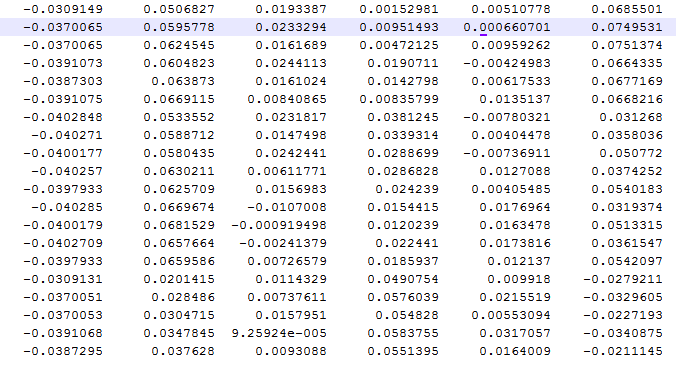
\includegraphics[scale=0.5]{EigenVectorsMeanValue.png}
   \caption{ Sniplet of eigenvectors matrix for the mean value weight method}	
 \end{figure}
 \begin{figure}[h!]
    \centering
    \label{fig:EigenVectorChosenMeanValueWeight}
    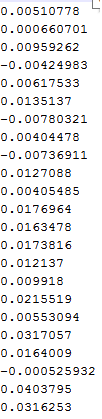
\includegraphics[scale=0.5]{EigenVectorChosenMeanValue.png}
    \caption{ Sniplet of the chosen eigenvector for the mean value coordinate method}	
  \end{figure}

\begin{figure}[h!]
   \centering
   \label{fig:eigenmeshmeanvalue}
   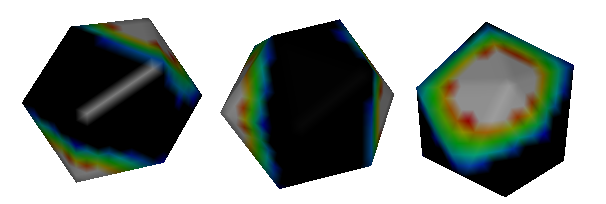
\includegraphics[scale=1]{EigenvectorMeshMeanValueCol4.png}
   \caption{ New mesh colormap based on the chosen $4_th$ column eigenvector for mean value coordinate method }	
 \end{figure}

Total time to finish the whole process is shown in Figure \ref{fig:computationtimeanvalue}.
\begin{figure}[h!]
   \centering
   \label{fig:computationtimeanvalue}
	\begin{lstlisting}[style=DOS]
	READ FILE
	Extension=WRL
	Reading IV/VRML
	Loading time :0.044 s
	P2P construction :0.008 s
	P2F construction :0.006 s
	F2F construction :0.056 s
	Egdes construction :0.035 s
	Write Laplacian matrix to text file.
	Calculating laplacian matrix: 2.663 s
	Computing Eigen decomposition
	Calculating eigen decomposition: 160.61 s
	Building eigen color map0.009 s
	Geodesic construction :0 s
	\end{lstlisting}
	\caption{Computation time}	
 \end{figure}


\end{homeworkProblem}


\newpage
\begin{homeworkProblem}[Section \arabic{homeworkProblemCounter} - Graphical User Interface]
This chapter will discuss on the development of the Graphical User Interface (GUI) to display what I have calculated previously. The implementation started with the $MeshLoader$ bundle given beforehand. $MeshLoader.pro$ is developed in $Qt SDK$. This bundle has already have many implementations that is extremely useful in developing this GUI. However, the $Widget$ is still missing in this bundle. I will extend the implementation of this bundle to include GUI, developed in $Qt Widget$ and cooperated Laplacian operators. 

First, I need to know what exactly classes in $MeshLoader$ do and try to use it in the new Widget application. 
There are 4 classes implemented. Below are a short description on what each of the classes do. 
\begin{enumerate}
\item $Mesh$ \\
 This class provides the base structure of the Mesh, which includes the vertices, faces, colors, textures, face normals, and vertex normals. The mesh stores each attribute in a $vector$ of $Vector3d$. This implementation use one of $C++$ Standard Template Library (STL), $vector$ class. It is z resizeable array that stores the datatype specified. The datatype used is from vector family of $Eigen$ library. Eigen library gives a convinient for matrix an vector manupulation which what we are dealing with. It also provides eigen solver that is very useful.
\item $NeighborMesh$ \\
 $NeighborMesh$ is a class inherited from $Mesh$ class. It has all the traits from $Mesh$, which means it will have all the vertices and faces stored, and also have additional traits defined in this class. Here, the surrounding environment of a vertex is computed. The neighborhood points , faces, edges, and distance are computed. I am mainly utilizing this class when computing the Laplacian.
\item $Scene$ \\
 This class provides functions to draw in $OpenGL$ ( camera position and lighting ) and handling user interaction ( like keyboard or ball tracking ). I will modified this class to support $QWidget$ for $OpenGL$ which is$ QGLWidget$. 
\item $Useful$
 This class provides some additional function that is used when calculating, rendering, or trying to corporate with C++.
\end{enumerate}


The Widget start with making the main window for the Application. The main file is very simple as, I only wants to instantiate $MainWindow$ class and show it out. The design of the window will be done in $ui$ file.
\codescript{main}{$Main.cpp$}

$MainWindow$ class acts as a base in my GUI. The button pushed, slider changed, check boxed checked will be registered in this class as slots. I can specified the post-processing of the action in these handler functions. The design in Qt is an xml-based UI, but Qt prohibits to directly changed the xml file, but instead use its designer interface. I utilized check boxes, radio buttons, buttons, horizontal sliders, and spin boxes.  

\begin{figure}[h!]
  \centering
  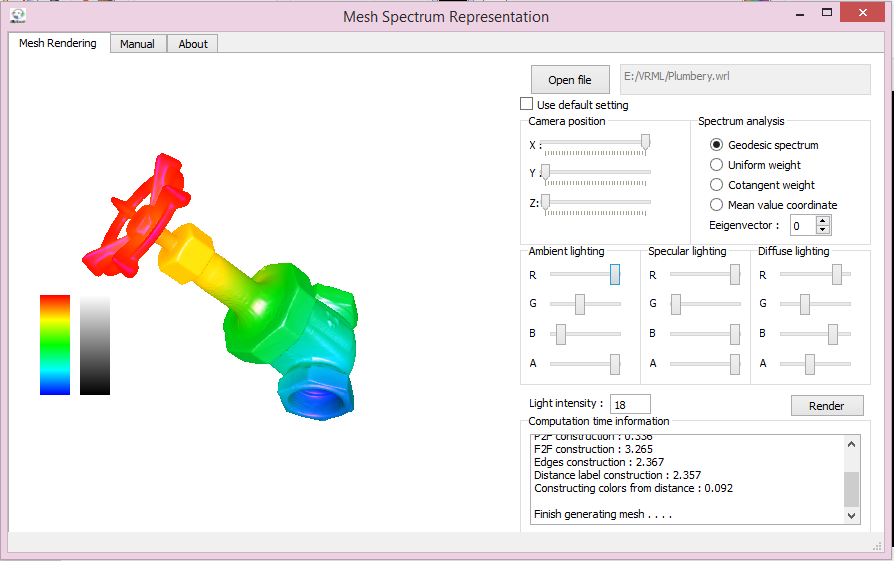
\includegraphics[scale=0.5]{MainWindow.png}
  \caption{Main window}
  \label{fig:mainwindow}
\end{figure}
\begin{figure}[h!]
  \centering
  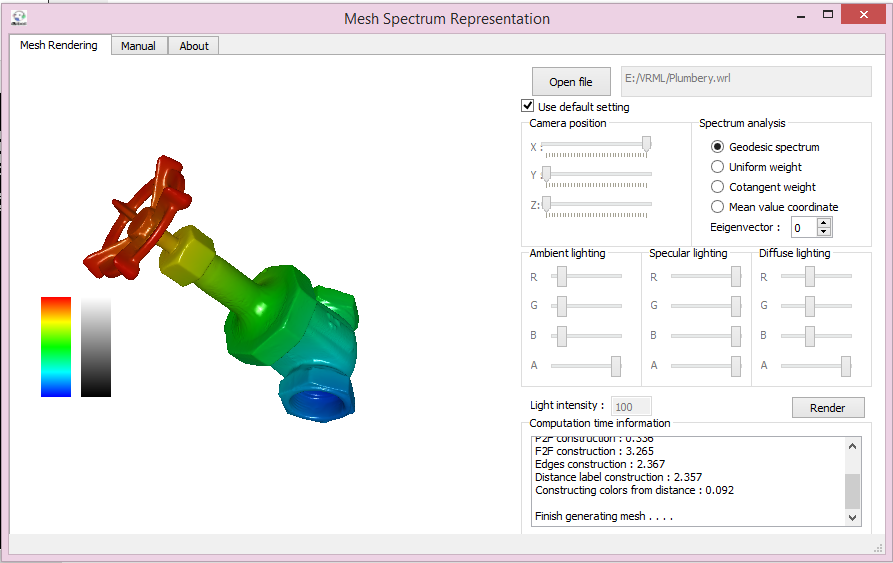
\includegraphics[scale=0.5]{MainWindowDefault.png}
  \caption{Default setting example}
  \label{fig:mainwindowdefault}
\end{figure}

As it shown in the main window, I have added the camera and lighting to be configurable from the interfaces. Checking the checkbox "Use default setting" will set the parameter to be the default setting of the application. Text box to show the computation time to generate the mesh also is added to give more information of the mesh rendering.

\codescript{mainWindowHeader}{Header file for  $MainWindow$ class}

One of the tricky part of the implementation is to cooperate OpenGL in QWidget. Having a very good reference from the class, I made $myGLWidget$ as the class on the widget to render the mesh. As shown in Figure \ref{fig:mainwindow}, area where the mesh is drawn is genereted from $myGLWidget$ class. 
\\
Now getting on the main problem which is rendering the 3D mesh to this area. As implemented in the bundle given, GLUT is used. I need to understand the Glut in C++ for this. GLUT is one of the OpenGL toolkit to implement GUI for OpenGL program. So, GLUT initiation and implementation will be done in $myGLWidget$ class. Figure

\codescript{myGLwidgetHeader}{Header file for  $myGLWidget$ class}
\codescript{myGLwidget}{$myGLWidget$ class}


The implementation of this class is a modification from $main.cpp$ and $Scene$ class from previous bundle. In here, I make all the initiation needed for GLUT rendering and as well handling the user interaction, such as $keyPressEvent$ and $mouseEvent$. It is worth noted that when making $keyPressEvent$, I need to set the focus for $myGLWidget$ to be $StrongFocus$. Otherwise, it will not execute the handler correctly. 

In order to make the camera position and lighting configurable, I make a new class $SceneGL$. This class handles the camera position and the lighting of the mesh rendering. 


\codescript{SceneGLHeader}{Header file for $SceneGL$ class}
\codescript{SceneGL}{$SceneGL$ class}

I use this class to store all of the camera and lighting related variables, update it when there is changes from the front page and render it back in the QGLWidget. Here I made all of the variables to be $private$ and make one public function for each of the variable. This class will be instantiated in $myGLWidget$ class. 
\\
Furthermore, I have added manual page directly in the widget to help the user to use the application. I notice that most of the standalone application built does not have a manual to be referred to and the shortcut is not mentioned eventhough there are great shortcuts have been implemented. I found this very inconvenient. I have added a short user manual in the application tab for this. 

\begin{figure}[h!]
  \centering
  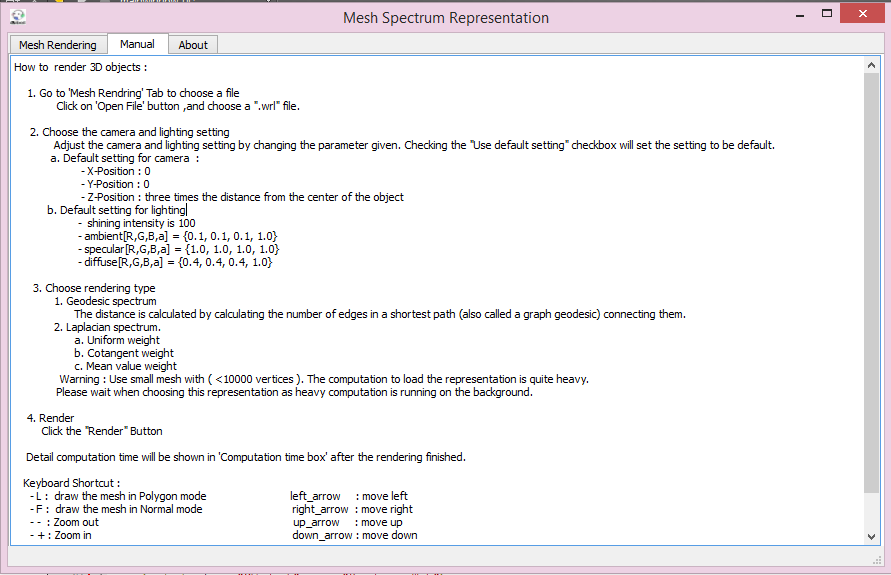
\includegraphics[scale=0.5]{ManualTab.png}
  \caption{Manual tab}
  \label{fig:manualtab}
\end{figure}
\begin{figure}[h!]
  \centering
  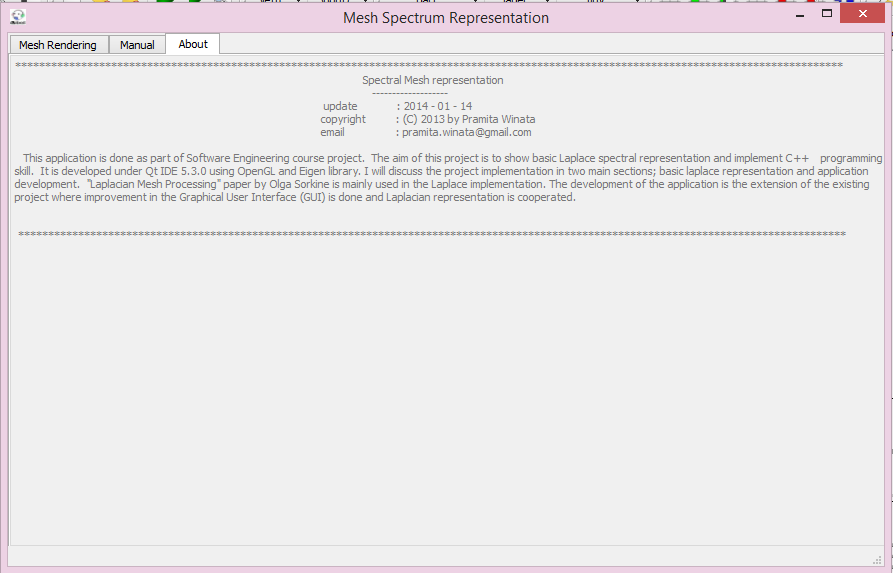
\includegraphics[scale=0.5]{AboutTab.png}
  \caption{About tab}
  \label{fig:abouttab}
\end{figure}
 

\end{homeworkProblem}
\newpage
\newpage
\begin{homeworkProblem}[Conclusion]
This project has been a very informative, useful, interesting, and tedious project. Not only that my programming skill is improved but also in researching scientific paper. Understanding Laplace operator is not as easy as it sounds. Reading many papers and researching need to be done to understand it. I have known C++ much better after implementing this project especially in integrating OpenGL and utilizing Eigen library. Not forget to mention, dealing with C++ standard library and overall behaviors are definitely very informative and useful. 
\end{homeworkProblem}

\begin{homeworkProblem}[Further Improvement]
\begin{itemize}
\item 
There are many improvements can be made to this application. In term of Laplacian representation, many additional features can be added, for example adding the anchor. Anchor implementation will enable us to get a deform mesh structure but still keeping the overall structure in place. This is definitely a very interesting and useful improvement. 
\item In the GUI point of view, many other additional features can be added, especially the implementation of Thread. I definitely noticed that rendering Laplacian representation takes a lot of time. It will be useful to implement a progress bar in order to show that the application actually is doing something in behind. A real time information also can be an option. 
\end{itemize}

\end{homeworkProblem}

\newpage

%Bibliographic references
\begin{thebibliography}{9}
\bibitem{laplacemesh} 
Olga Sorkine,\textit{“Laplacian Mesh Processing}. 
STAR report, Eurographics, 2005.

\bibitem{meshpro} 
Mesh Processing, G. Peyré,
\\\texttt{ https://www.ceremade.dauphine.fr/~peyre/teaching/manifold-sci/}

\bibitem{eigenlib} 
Eigen library,
\\\texttt{ http://eigen.tuxfamily.org/index.php?title=Main\_Page } 

\bibitem{c++lib}
The C++ Standard library, see\\\texttt{ http://www.yolinux}.

\bibitem{cotangentweight}
MEYER M., DESBRUN M., SCHRÖDER P.,
BARR A. H.: Discrete differential-geometry operators for
triangulated 2-manifolds. In \textit{“Visualization and Mathematics
III}, Hege H.-C., Polthier K., (Eds.). Springer-Verlag,
Heidelberg, 2003, pp. 35–57.

\bibitem{areatriangle}
HERON. 60. \\\texttt{Metrica}. Alexandria, Roman Egypt.

\bibitem{conGraph}
FIEDLER M.: Algebraic connectivity of graphs.
\\\texttt{Czech. Math. Journal 23 }(1973), 298–305.

\bibitem{meanValue}
LOATER M. S.: Mean value coordinates. \\\texttt{ CAGD 20}, 1 (2003), 19–27.
\end{thebibliography}

\end{document}